% =====================================================================
% figB  — R/ggplot2 -> tikzDevice (parallel to ../figures-tex/figB_surrogate.tex)
% Canonical-JSON-only. Regenerate: Rscript figures/make_figures_ieee.R
% Provenance (JSON path :: field = plotted value), one line per series:
% SOURCE: results/C1_mechanism_sc_table.json :: groups[llama1b,L8].within_probe_rho_SC = 0.4015
% SOURCE: results/G2_gradsim_L8.json :: aggregate.gradsim_within_probe.resid.mean = 0.3899
% SOURCE: results/C1_mechanism_sc_table.json :: groups[llama1b,L10].within_probe_rho_SC = 0.5526
% SOURCE: results/G2_gradsim_L10.json :: aggregate.gradsim_within_probe.resid.mean = 0.5279
% SOURCE: results/C1_mechanism_sc_table.json :: groups[llama1b,L12].within_probe_rho_SC = 0.6765
% SOURCE: results/G2_gradsim_L12.json :: aggregate.gradsim_within_probe.resid.mean = 0.6277
% SOURCE: results/C1_mechanism_sc_table.json :: groups[llama1b,L14].within_probe_rho_SC = 0.5037
% SOURCE: results/G2_gradsim_L14.json :: aggregate.gradsim_within_probe.resid.mean = 0.4981
% =====================================================================
% !TEX encoding = UTF-8 Unicode
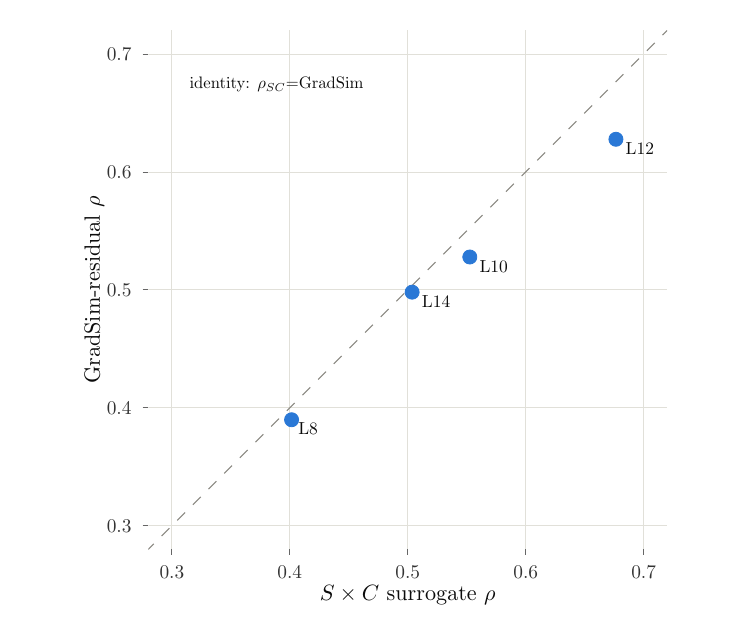
\begin{tikzpicture}[x=1pt,y=1pt]
\definecolor{fillColor}{RGB}{255,255,255}
\path[use as bounding box,fill=fillColor,fill opacity=0.00] (0,0) rectangle (252.94,209.58);
\begin{scope}
\path[clip] ( 19.84,  0.00) rectangle (233.10,209.58);
\definecolor{fillColor}{RGB}{255,255,255}

\path[fill=fillColor] ( 19.84,  0.00) rectangle (233.10,209.58);
\end{scope}
\begin{scope}
\path[clip] ( 43.58, 21.06) rectangle (231.10,208.58);
\definecolor{drawColor}{RGB}{225,224,217}

\path[draw=drawColor,line width= 0.3pt,line join=round] ( 43.58, 29.59) --
	(231.10, 29.59);

\path[draw=drawColor,line width= 0.3pt,line join=round] ( 43.58, 72.20) --
	(231.10, 72.20);

\path[draw=drawColor,line width= 0.3pt,line join=round] ( 43.58,114.82) --
	(231.10,114.82);

\path[draw=drawColor,line width= 0.3pt,line join=round] ( 43.58,157.44) --
	(231.10,157.44);

\path[draw=drawColor,line width= 0.3pt,line join=round] ( 43.58,200.06) --
	(231.10,200.06);

\path[draw=drawColor,line width= 0.3pt,line join=round] ( 52.11, 21.06) --
	( 52.11,208.58);

\path[draw=drawColor,line width= 0.3pt,line join=round] ( 94.72, 21.06) --
	( 94.72,208.58);

\path[draw=drawColor,line width= 0.3pt,line join=round] (137.34, 21.06) --
	(137.34,208.58);

\path[draw=drawColor,line width= 0.3pt,line join=round] (179.96, 21.06) --
	(179.96,208.58);

\path[draw=drawColor,line width= 0.3pt,line join=round] (222.58, 21.06) --
	(222.58,208.58);
\definecolor{drawColor}{RGB}{137,135,129}

\path[draw=drawColor,line width= 0.4pt,dash pattern=on 4pt off 4pt ,line join=round] (-143.94,-166.46) -- (418.62,396.10);
\definecolor{drawColor}{RGB}{42,120,214}
\definecolor{fillColor}{RGB}{42,120,214}

\path[draw=drawColor,line width= 0.3pt,line join=round,line cap=round,fill=fillColor] ( 95.36, 67.90) circle (  2.54);

\path[draw=drawColor,line width= 0.3pt,line join=round,line cap=round,fill=fillColor] (159.76,126.71) circle (  2.54);

\path[draw=drawColor,line width= 0.3pt,line join=round,line cap=round,fill=fillColor] (212.56,169.25) circle (  2.54);

\path[draw=drawColor,line width= 0.3pt,line join=round,line cap=round,fill=fillColor] (138.92,114.01) circle (  2.54);
\definecolor{drawColor}{RGB}{11,11,11}

\node[text=drawColor,anchor=base west,inner sep=0pt, outer sep=0pt, scale=  0.63] at ( 97.80, 62.40) {L8};

\node[text=drawColor,anchor=base west,inner sep=0pt, outer sep=0pt, scale=  0.63] at (163.29,121.21) {L10};

\node[text=drawColor,anchor=base west,inner sep=0pt, outer sep=0pt, scale=  0.63] at (216.09,163.74) {L12};

\node[text=drawColor,anchor=base west,inner sep=0pt, outer sep=0pt, scale=  0.63] at (142.45,108.51) {L14};

\node[text=drawColor,anchor=base west,inner sep=0pt, outer sep=0pt, scale=  0.60] at ( 58.50,187.46) {identity: $\rho_{SC}{=}$GradSim};
\end{scope}
\begin{scope}
\path[clip] (  0.00,  0.00) rectangle (252.94,209.58);
\definecolor{drawColor}{gray}{0.20}

\node[text=drawColor,anchor=base east,inner sep=0pt, outer sep=0pt, scale=  0.70] at ( 37.53, 27.31) {0.3};

\node[text=drawColor,anchor=base east,inner sep=0pt, outer sep=0pt, scale=  0.70] at ( 37.53, 69.93) {0.4};

\node[text=drawColor,anchor=base east,inner sep=0pt, outer sep=0pt, scale=  0.70] at ( 37.53,112.54) {0.5};

\node[text=drawColor,anchor=base east,inner sep=0pt, outer sep=0pt, scale=  0.70] at ( 37.53,155.16) {0.6};

\node[text=drawColor,anchor=base east,inner sep=0pt, outer sep=0pt, scale=  0.70] at ( 37.53,197.78) {0.7};
\end{scope}
\begin{scope}
\path[clip] (  0.00,  0.00) rectangle (252.94,209.58);
\definecolor{drawColor}{gray}{0.40}

\path[draw=drawColor,line width= 0.3pt,line join=round] ( 41.58, 29.59) --
	( 43.58, 29.59);

\path[draw=drawColor,line width= 0.3pt,line join=round] ( 41.58, 72.20) --
	( 43.58, 72.20);

\path[draw=drawColor,line width= 0.3pt,line join=round] ( 41.58,114.82) --
	( 43.58,114.82);

\path[draw=drawColor,line width= 0.3pt,line join=round] ( 41.58,157.44) --
	( 43.58,157.44);

\path[draw=drawColor,line width= 0.3pt,line join=round] ( 41.58,200.06) --
	( 43.58,200.06);
\end{scope}
\begin{scope}
\path[clip] (  0.00,  0.00) rectangle (252.94,209.58);
\definecolor{drawColor}{gray}{0.40}

\path[draw=drawColor,line width= 0.3pt,line join=round] ( 52.11, 19.06) --
	( 52.11, 21.06);

\path[draw=drawColor,line width= 0.3pt,line join=round] ( 94.72, 19.06) --
	( 94.72, 21.06);

\path[draw=drawColor,line width= 0.3pt,line join=round] (137.34, 19.06) --
	(137.34, 21.06);

\path[draw=drawColor,line width= 0.3pt,line join=round] (179.96, 19.06) --
	(179.96, 21.06);

\path[draw=drawColor,line width= 0.3pt,line join=round] (222.58, 19.06) --
	(222.58, 21.06);
\end{scope}
\begin{scope}
\path[clip] (  0.00,  0.00) rectangle (252.94,209.58);
\definecolor{drawColor}{gray}{0.20}

\node[text=drawColor,anchor=base,inner sep=0pt, outer sep=0pt, scale=  0.70] at ( 52.11, 10.46) {0.3};

\node[text=drawColor,anchor=base,inner sep=0pt, outer sep=0pt, scale=  0.70] at ( 94.72, 10.46) {0.4};

\node[text=drawColor,anchor=base,inner sep=0pt, outer sep=0pt, scale=  0.70] at (137.34, 10.46) {0.5};

\node[text=drawColor,anchor=base,inner sep=0pt, outer sep=0pt, scale=  0.70] at (179.96, 10.46) {0.6};

\node[text=drawColor,anchor=base,inner sep=0pt, outer sep=0pt, scale=  0.70] at (222.58, 10.46) {0.7};
\end{scope}
\begin{scope}
\path[clip] (  0.00,  0.00) rectangle (252.94,209.58);
\definecolor{drawColor}{RGB}{11,11,11}

\node[text=drawColor,anchor=base,inner sep=0pt, outer sep=0pt, scale=  0.80] at (137.34,  2.73) {$S\times C$ surrogate $\rho$};
\end{scope}
\begin{scope}
\path[clip] (  0.00,  0.00) rectangle (252.94,209.58);
\definecolor{drawColor}{RGB}{11,11,11}

\node[text=drawColor,rotate= 90.00,anchor=base,inner sep=0pt, outer sep=0pt, scale=  0.80] at ( 26.05,114.82) {GradSim-residual $\rho$};
\end{scope}
\end{tikzpicture}
